\section{Detailed Design Optical Emitting Payload} 
\label{sec:DDlaser}
\acs{LiDAR} is a remote sensing system comprising an optical emitting device, used to acquire topographic data, e.g. surface elevation gradients or ground composition by evaluating the \acs{BRDF}, considering multi-angular measurement are taken. For the generation of optical pulses, a highly efficient, diode-pumped, solid-state Nd-YAG \acs{laser} is considered \ac{DPSSL}. Solid-State \acp{laser} have a high \acs{TRL} with relatively good properties in terms of beam quality (Q-factor), efficiency and pulse manipulation. 

\subsection{Diode Laser Characteristics}
\label{laser_diodes}
\acs{laser} diodes are electrically pumped semiconductor \acp{laser}, in which the gain is generated by an electrical current flowing through a \textit{p-n junction} or (more frequently) a \textit{p-i-n structure}. In such a heterostructure, excitons dynamics can occur (electrons and holes can recombine), releasing the energy portions as photons. This process can be spontaneous, but can also be stimulated by incident photons, in effect leading to optical amplification. Most higher-power \acs{laser} diodes, however, exhibit a relatively poor beam quality, combined with other non-favorable properties, such as a large beam divergence, high asymmetry of beam radius and beam quality between two perpendicular directions, and astigmatism (property of rays to exhibit different foci in different symmetrical planes). Especially considering the long distances used in \acs{LiDAR} missions, these properties degrade the potential data quantity, as well as quality. In this \acs{laser} configuration the diode laser is used as input (or pump) energy for the solid-state laser.

\acs{laser} diodes are electrically pumped semiconductor \acp{laser}, in which the gain is generated by an electrical current flowing through a \textit{p-n junction} or (more frequently) a \textit{p-i-n structure}. In such a heterostructure, excitons dynamics can occur (electrons and holes can recombine), releasing the energy portions as photons. This process can be spontaneous, but can also be stimulated by incident photons, in effect leading to optical amplification. Most higher-power \acs{laser} diodes, however, exhibit a relatively poor beam quality, combined with other non-favorable properties, such as a large beam divergence, high asymmetry of beam radius and beam quality between two perpendicular directions, and astigmatism (property of rays to exhibit different foci in different symmetrical planes). Especially considering the long distances used in \acs{LiDAR} missions, these properties degrade the potential data quantity, as well as quality. In this \acs{laser} configuration the diode laser is used as input (or pump) energy for the solid-state laser.

picture!!!

A quantum well is a thin layer which can confine (quasi-)particles (typically electrons or holes) in the dimension perpendicular to the layer surface, whereas the movement in the other dimensions is not restricted. A quantum well is often realized with a thin layer of a semiconductor medium, embedded between other semiconductor layers of wider bandgap. The thickness of such a quantum well is typically $\sim$5-20 [nm]. The choice of semiconductor layer material gives rise to specific wavelength generation. For the specific wavelength of interest ($\sim$946 [nm]), an Indium gallium arsenide (InGaAs) quantum well embedded in Gallium Arsenide (GaAs), is chosen, which shows wavelength propagation in the interval 900 - 1000 [nm]. 

A major challenge is to reach the laser threshold, because the optical gain for the intracavity laser beam occurs only on a very small distance (in one or several quantum wells). It is therefore necessary to realize a laser resonator with very low losses, i.e., \textit{Bragg mirrors} with high reflectivity. A Bragg mirror (also called \textit{distributed Bragg reflector}) is a structure which consists of an alternating sequence of layers of two different optical materials. The principle of operation can be understood as follows. Each interface between the two materials contributes a Fresnel reflection. For the design wavelength, the optical path length difference between reflections from subsequent interfaces is half the wavelength; in addition, the reflection coefficients for the interfaces have alternating signs. Therefore, all reflected components from the interfaces interfere constructively, which results in a strong reflection. The reflectivity achieved is determined by the number of layer pairs and by the refractive index contrast between the layer materials. 
Individual \acs{laser} diodes normally generate continuous waves with powers $\sim$ 1 - 10 [mW]. To be able to generate higher power ($\sim$1 - 10 [W]) \textit{laser diodes arrays} or \textit{laser diode stacks} can be created, simply be combining multiple individual \acs{laser} diodes.

\begin{figure} [ht]
\centering
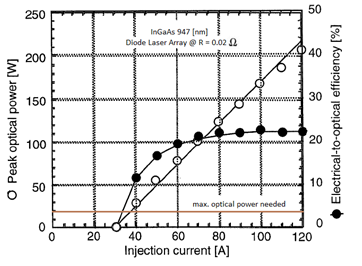
\includegraphics[scale=1.2]{chapters/img/laser_power.png}	
\caption{laser power \cite{laser_power} }
\label{laser_power}
\end{figure}

\subsection{Diode Pumped Solid-State Laser Configuration} 
\label{laserconfig}
introduction

\subsubsection{Nd-YAG Laser Characteristics}
\label{nd_yag}
\textit{Yttrium Aluminum Garnet} has emerged as the most widely produced laser gain host and has enjoyed recent popularity as a substrate material for optical components. The YAG host is a stable compound, mechanically robust, physically hard, optically isotropic, and transparent from below 300 to beyond 4,000 [nm]. YAG single crystals are able to accept trivalent laser activator ions from both the rare Earth and transition metal groups, and can be grown with very low strain.

The Nd-YAG laser did not become a widely accepted tool until the 1970s, finding its first important application in the laser rangefinder arena. These YAG systems could be run at higher repetition rates, higher output energies,  
and operate more covertly than the first generation ruby systems, primarily because of the thermal stability and robust nature of the Nd-YAG material. After gaining acceptance within the military community, the scientific, industrial, and medical markets were explored. Nd-YAG lasers quickly gained recognition in new market applications due to their increased reliability and flexibility in delivery of the laser beam via fiber optics.

For applications where TEM00 single mode operation is required, it is necessary to reduce or eliminate the variations in the bulk material and in the absorption of the pumping radiation throughout the component. In addition, wavefront distortions due to geometric imperfections and thermal gradient effects such as thermal lensing must be minimized. In this case, Neodymium concentration in the 0.4 to 0.8\% range is typically specified.

\begin{figure} [ht]
\centering
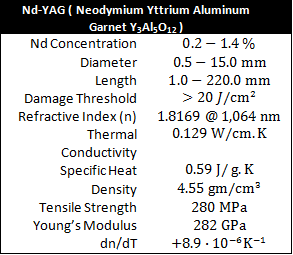
\includegraphics[scale=1.2]{chapters/img/laser_configuration.png}	
\caption{laser configuration}
\label{laser}
\end{figure}

\begin{figure} [ht]
\centering
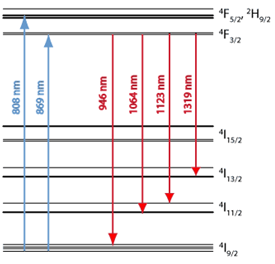
\includegraphics[scale=1.2]{chapters/img/laser_line.png}	
\caption{laser line}
\label{laser}
\end{figure}

\subsubsection{Second Harmonic Generation}
\label{SHG}
Since Nd-YAG has no principle absorption peak at the desired wavelength for the \acs{LiDAR} mission, the frequency should be altered from the original 946 [nm]. This can be done using \textit{second harmonic generation} or \textit{frequency doubling} in nonlinear crystals.
The physical mechanism behind frequency doubling can be understood as follows. Due to the ��(2) nonlinearity, the fundamental (pump) wave generates a nonlinear polarization wave which oscillates with twice the fundamental frequency. According to Maxwell's equations, this nonlinear polarization wave radiates an electromagnetic field with this doubled frequency. Due to phase-matching issues (see below), the generated second-harmonic field propagates dominantly in the direction of the nonlinear polarization wave. The latter also interacts with the fundamental wave, so that the pump wave can be attenuated (pump depletion) when the second-harmonic intensity develops: energy is transferred from the pump wave to the second-harmonic wave.

\subsubsection{Pulse Generation}
\label{pockel}
The generation and manipulation of pulses can highly influent the data in \acs{LiDAR} missions. To be able to transform the continuous wave into a pulsed wave, Q-switching is applied. Q-switching is a technique for obtaining energetic short pulses from a laser by modulating the intracavity losses and thus the Q-factor (a measure of the damping of resonator modes) of the laser resonator. The technique is mainly applied for the generation of nanosecond pulses of high energy and peak power with solid-state bulk lasers. For \textit{active Q-switching}, the losses are modulated with an active control element typically either an acousto-optic or electro-optic modulator. Both techniques rely on the fact that the optical properties within a nonlinear crystal change on the occurrence of an induced sound wave (acousto-optic) or electric field (electro-optic). There are also mechanical Q-switches such as spinning mirrors, used as end mirrors of laser resonators. In any case, the achieved pulse energy and pulse duration depends on the energy stored in the gain medium, i.e. on the pump power and the pulse repetition rate.  A Pockels cell is a device consisting of an electro-optic crystal (with some electrodes attached to it) through which a light beam can propagate. Dependent on the configuration, the phase delay or polarization state in the crystal (due to the \textit{Pockels effect}) can be modulated by applying a variable electric voltage.  Hence, for short periods (dt) the polarization state of the incoming electromagnetic radiation can be altered. If a \textit{polarizer disk} is used after the Pockel cell, the generation of pulses will begin, since the polarizer disk transmits certain polarized states only, deflecting the rest (acting like a 'polarize filter'). Pulses in the order of nanoseconds could be created this way. Care should be taken at the fact that the peak power after the Pockel cell is increased in several orders, due to the conversion from continuous to pulsed waves. Hence, the polarizer disk should be able to cope with these stresses.

\begin{figure} [ht]
\centering
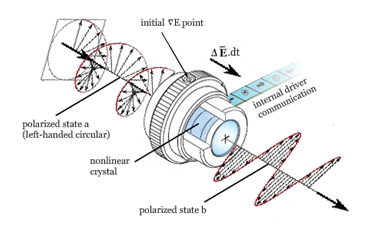
\includegraphics[scale=1.2]{chapters/img/laser_polarized.png}	
\caption{laser polarized}
\label{laser}
\end{figure}

\subsection{Optical Characteristics} 
\label{opticalchar}
The radius of the beam equals 400 [$\mu$m]. Considering a $TEM_{00}$ transverse mode of electromagnetic radiation this results in a area equal to 
\begin{equation}
\label{area}
A_{beam} = \pi \cdot r^{2} = \pi \cdot 400^{2} = 502,654 \mu m^{2} = 0.50265 cm^{2}
\end{equation}

The pulse energy $E_{p}$ [J] (maximum optical power of a pulse) is determined using the simulator. Sufficient energy should be present within the electromagnetic radiation to ensure the optimum path from the transmitter towards the receiver. Lowering the value of $E_{p}$ below this threshold energy can lead to atmospheric and surface absorption or translational mismatching due to incorrect scattering. The value of $E_{p}$ of this particular mission is determined to be $\sim$1 [mJ] (see \ref{simulator}).
Pulse repetition rate $f_{rep}$ [Hz], i.e. the number of pulses emitted per second, is an important parameter for the altimetry mission. Again, using the results from the simulator, the quantity of this parameter can be determined to be $\sim$5000 [Hz] ($\Delta$t = 0.0002 [s] with a pulse duration $t_{p}$ $\sim$10 [ns]). Using the value of $f_{rep}$, the spatial resolution of the pulses along-track and in the nadir-direction can be calculated, considering the orbital velocity to be fixed at the determined altitude.  
\begin{equation}
\label{alongtrackres}
d_{along} = \Delta t \cdot v = 0.0002 [s] \cdot 7,617 [m/s] = 1.5234 [m]
\end{equation}

\begin{equation}
\label{alongtracknadir}
d_{nadir} = \Delta t \cdot c = 0.0002 [s] \cdot 299,792,458 [m/s] = 59,958.49 [m]
\end{equation}

Considering the value of $E_{p}$ to be 1 [mJ] with a $f_{rep}$ of 5,000 [Hz], the total power that should be induced within the electromagnetic wave can be calculated.
\begin{equation}
\label{outputpower}
P_{output} = E_{p} \cdot f_{rep} = 0.001 [J] \cdot 5,000[1/s] = 5.0 [W]
\end{equation}

Input power equals output power times efficiency = $16 W \times eff = ((0.35)*(0.99)^6)$
The pulse peak intensity equals $E_{p}/t_{p} = 0.001 [J] / 10\cdot10^{-9} [s] = 100,000 W$. The intensity turns out to be $\frac{E_{p}/t_{p}}{A_{beam}} = \frac{100,000 [W]}{0.50265 [cm^{2}]} = 198,950.6 [W/cm^{2}] (0.00199 [J/cm^{2}/10ns])$. The standard damage threshold energy $E_{p,damage}$for dielectric components equals $0.5 - 10 [J/cm^{2}/10 ns]$. Considering the lowest value $I_{p,damage}$, hence, $0.5 [J/cm^{2}/10 ns]$, and converting this to the appropriate dimensions, shows the intensity created within the electromagnetic pulses should do no harm to the dielectric components. Especially the polarizer disk (with the lowest $I_{p,damage}$) is vulnerable for peak power caused by pulsed electromagnetic radiation. 

\subsection{Thermal Control} 
\label{opticalthermal}
content!!

\subsection{ Laser Lifetime Expectance} 
\label{opticallifetime}
Considering a constant value of $f_{rep}$, the total number of pulses sent per year equals $1.5768\cdot10^{11}$ [pulses/year]. All optical components should be able to cope with the large amount of pulses and the peak power implied by these pulses, i.e. the energy damage threshold of the dielectric components should be higher than the incoming energy of the electromagnetic radiation. Since $I_{p,damage}$) is given with a temporal resolution in the order of a single pulse width ($\sim$10 [ns]), individual pulses can be analyzed. Stationary calculations can be conducted with the information based on the electromagnetic radiation energy and hence, the proper optical elements could be chosen ($I_{p,damage} > I_{p}$).
\ref{} shows an experimental set-up, where the lifetime of a \acs{DPSSL} is investigated, using approximately the same \acs{laser} configuration with $f_{rep}$ = 242 [Hz] and $E_{p}$ = 0.0150 [J]. The pulse energy is much larger then the value of $E_{p}$ in the case of the \acs{LIDAR} mission described in this report ($\sim$0.001 [J]). \ref{figure} shows the results.

%\begin{figure}[ht!]
%\centering
%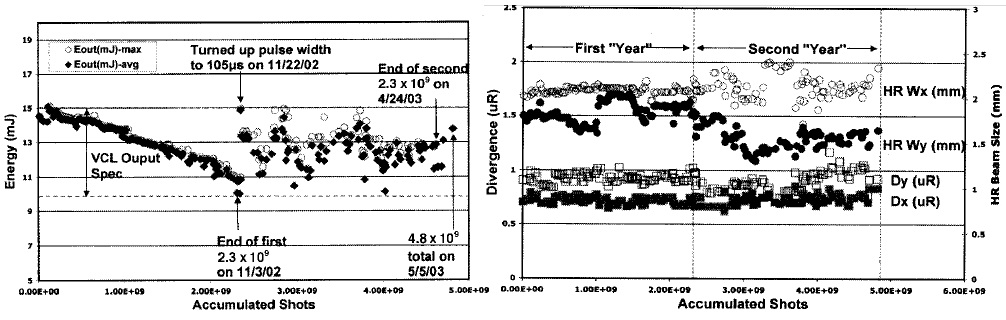
\includegraphics[scale=0.5]{chapters/img/Nd-YAG_reliability.jpg} 
%\caption{}
%\label{reliability}
%\end{figure}
